% This is a comment, this will be not be read by the machine

% Which type of document do you want?
\documentclass[a4paper,12pt]{article} 

% Use packages for different functioanlities
\usepackage[utf8]{inputenc} % For character encoding
\usepackage{natbib} % For bibliography
\usepackage{amsmath} % For mathematics
\usepackage{amssymb}
\usepackage{graphicx} % For graphics
\usepackage{url} % For including web links
\usepackage{tikz} % For advanced graphics with the language TikZ
\usepackage[font=footnotesize]{caption} 
\linespread{1.33} % Control spread between lines
\usepackage[toc,page]{appendix} 
\usepackage[colorlinks=true,linkcolor=red,urlcolor=red,citecolor=blue,backref=page]{hyperref} 
\usepackage{rotating}
\usepackage{amsthm}
% \usepackage[top=2.5cm, bottom=2.5cm, left=3cm, right=3cm]{geometry}

% Now comes the main part
\title{Introduction to \LaTeX\\
\scriptsize{Put subtitle here}} %This sets up the title, note the `\\' command for a newline
%\title{new title}
\author{Abhinav Anand}
%\thanks{Herein goes thanks.}

\date{} %If you comment this out, the date will be displayed

\begin{document}

\maketitle %This command "makes" the title

\begin{abstract}

Ha ha ha what a funny abstract!

\end{abstract}

\section{What a funny section!}
\label{Funny_Label}

\LaTeX uses a ``markup language'' in order to convert text, combined with the markup, into a high quality document. For example, web pages work in a similar way: the HTML 
(Hyper Text Markup Language) is used to style the text document, and the browser presents it in its full glory --- with different colors, fonts, sizes, etc.
%\\\\\\
Each of the \LaTeX commands begin with a backslash. This is \LaTeX's way of knowing that whenever it sees a backslash, to expect some commands. Comments are not classed as a commands.

You can force a new line using \\
%To force a new page, use \newpage or \clearpage

this is the ``right'' way

this is the ''wrong'' way

\section*{The section with no number}

That's how you do it --- with a star!

\subsection{Subsection}

Here is my subsection

In order to have a subsection without a name, just use the old trick --- attach
a star to the end of the command: %\subsection*{}

\subsubsection{This is my subsubsection}

Again, use the star in the relevant command to omit natural numbering of sections.

Now let us introduce equations, since that's what we're here to learn!

\section{Support for Mathematics}

You can generate equations via the following ``environment'' --- the 
equation environment enclosed in the ``begin'' and ``end'' equations:
% (Note the biggest mistake made in latex when enclosing quotes: `` vs '')$ \dfrac{num}{den} $

\begin{equation}
\label{Eq:Number_1}
\int_{0}^{\infty} e^{-\rho} \rho^{2l}\left[ L_{n+l}^{2l+1} \left(\rho
\right) \right]^2 \rho^2 d\rho = \frac{2n \left[\left(n+l\right)!
	\right]^3}{(n-l-1)!}
\end{equation}

$\displaystyle\sum_{i=0}^{i=\infty}f^2$

Needless to say you can generate any equation of any arbitrary complexity and it is 
guaranteed to be rendered beautifully.

If you don't want the equation numbers you can use a star after the word 
``equation'' above. TeXstudio prompts you anyway regarding that.

Yet another way to generate anonymous equations is the following operator: %\[\]

\[
\bar{N}_j^g = \frac{\sum\limits_{k} N_{jk} W_k}{\sum\limits_{K} W_k}
\]




You can also use equations inline by using the dollar signs and squeezing all
mathematics within them. For example, $\nexists$ a markup/typesetting language
better than \LaTeX  and it's as easy to see as $x^2 + x_1 + x = g(\cdot)$.\footnote{Let's add a footnote for fun!}

\subsection{Subequations}

Let's now add subequations to complete the discussion

\begin{subequations}
	\begin{equation}
	e^{i\pi} + 1 = 0
	\label{1a}
	\end{equation}
	\begin{equation}
	\nabla \times \mathbf{H} = \frac{\varepsilon}{c} \frac{\partial \mathbf{E}}{\partial{t}}
	\label{1b}
	\end{equation}
	\label{1}
\end{subequations}

More mathematics:


$\sqrt[3]{5}$

$\frac{x}{y}$

$\dfrac{\displaystyle\int_{0}^{\infty}fg d\mu}{\frac{\varepsilon}{c}}$

$A^{x} {y}$

$\sum {k=1}^n k$

$2 \ne 4$

$\phi \in \Psi$

$\hat{\i} \times \hat{\j} = \hat{k}$

$f^{\prime}(\xi)$

180$^{\circ}$C


\section{Figures}

To include figures in a document the package graphicx is required, so the command
%\usepackage{graphicx} 
must be written in the preamble. To add a figure one can
write the following commands.

 \begin{figure}[h!tbp] % htbp
 	\centering
 	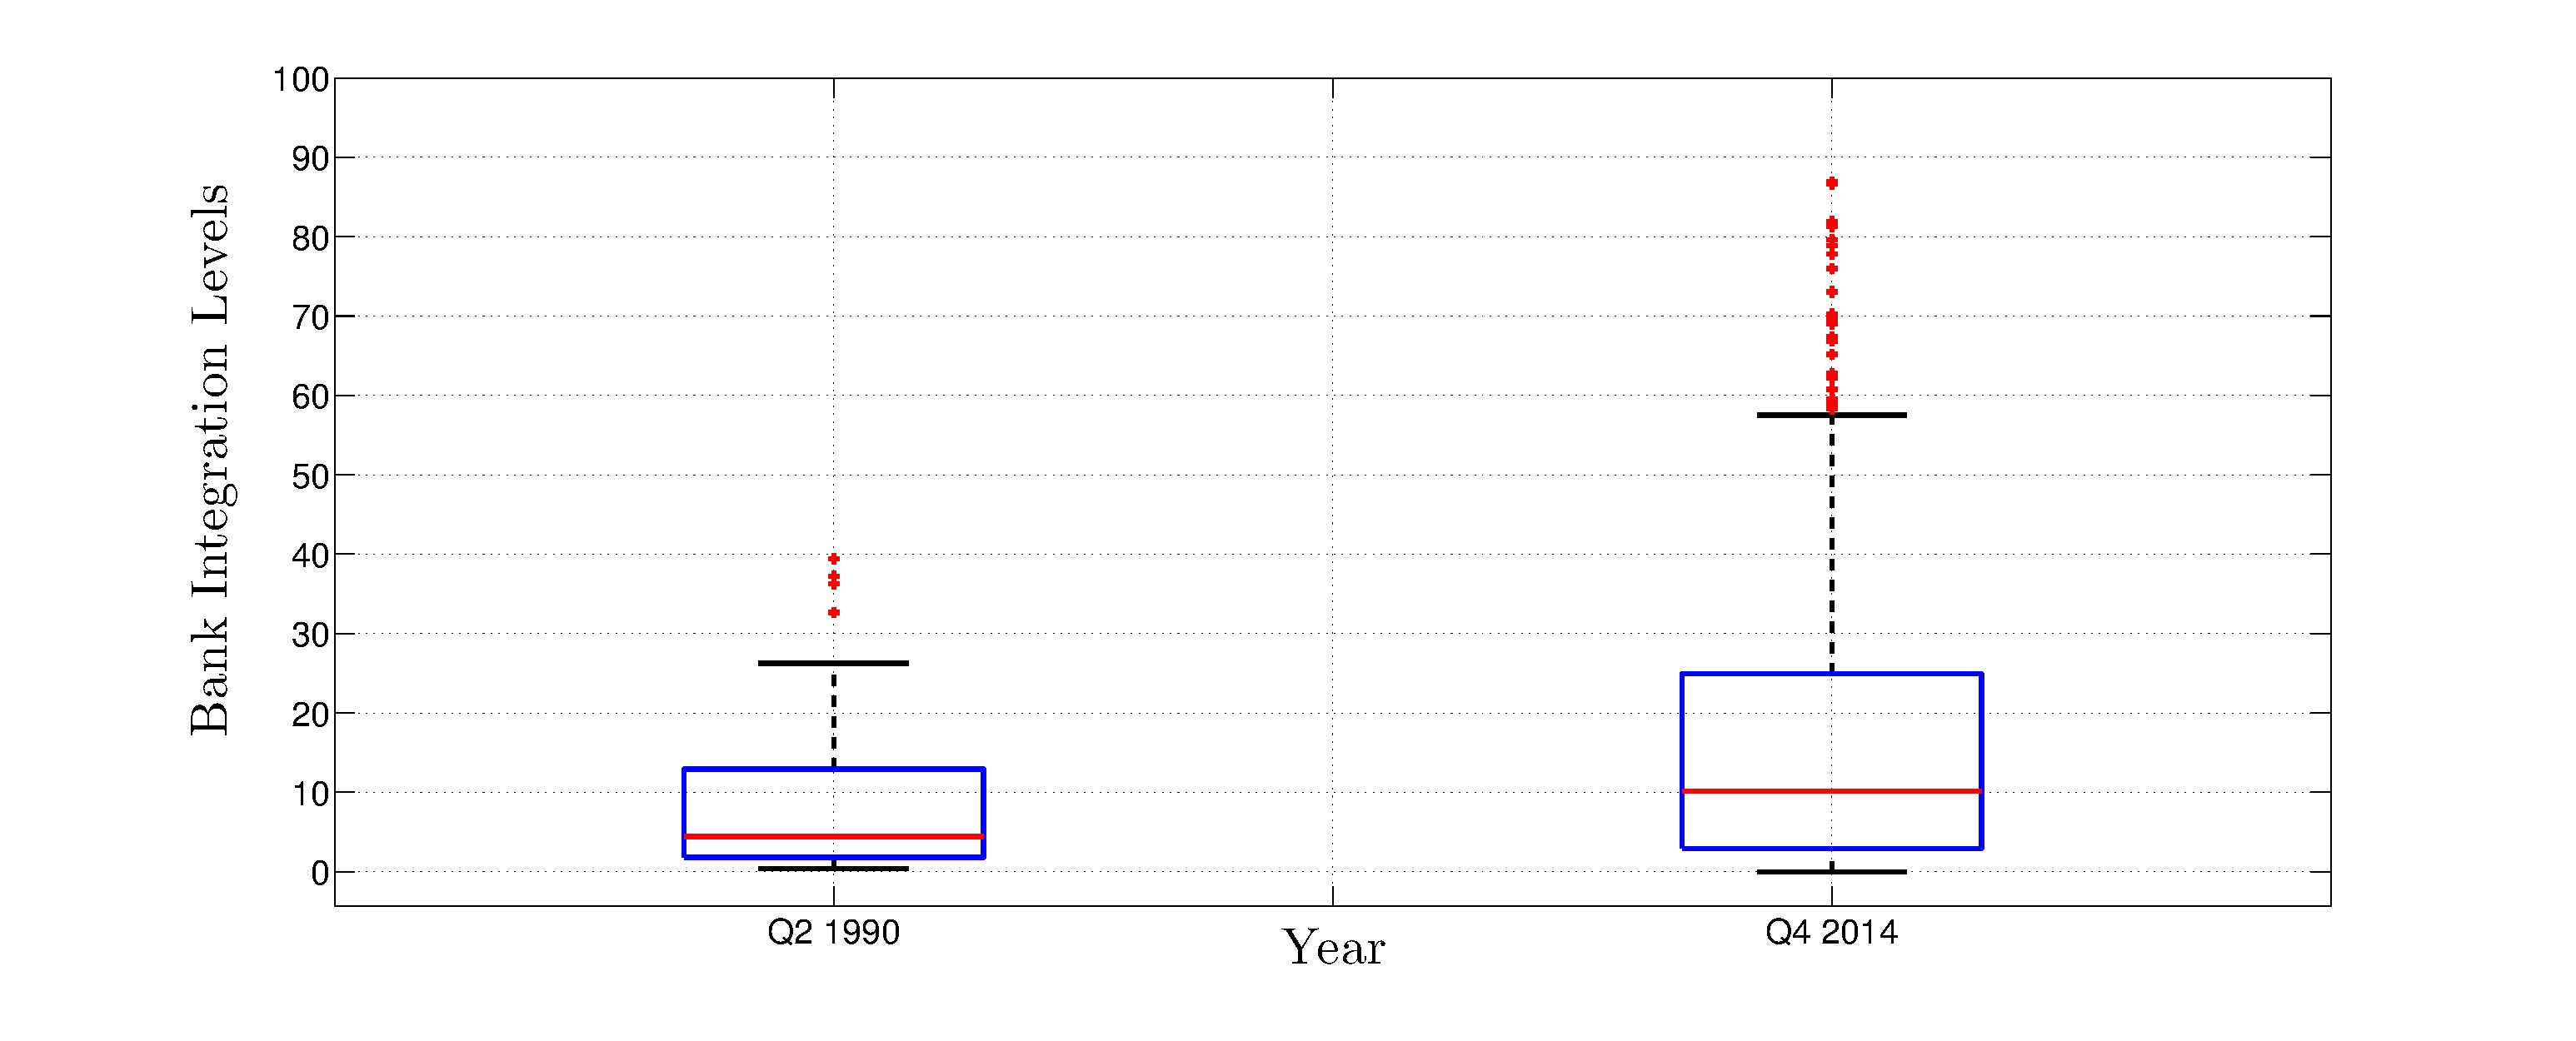
\includegraphics[width=12cm,height=6cm]{Boxplot_Integration.pdf}
 	%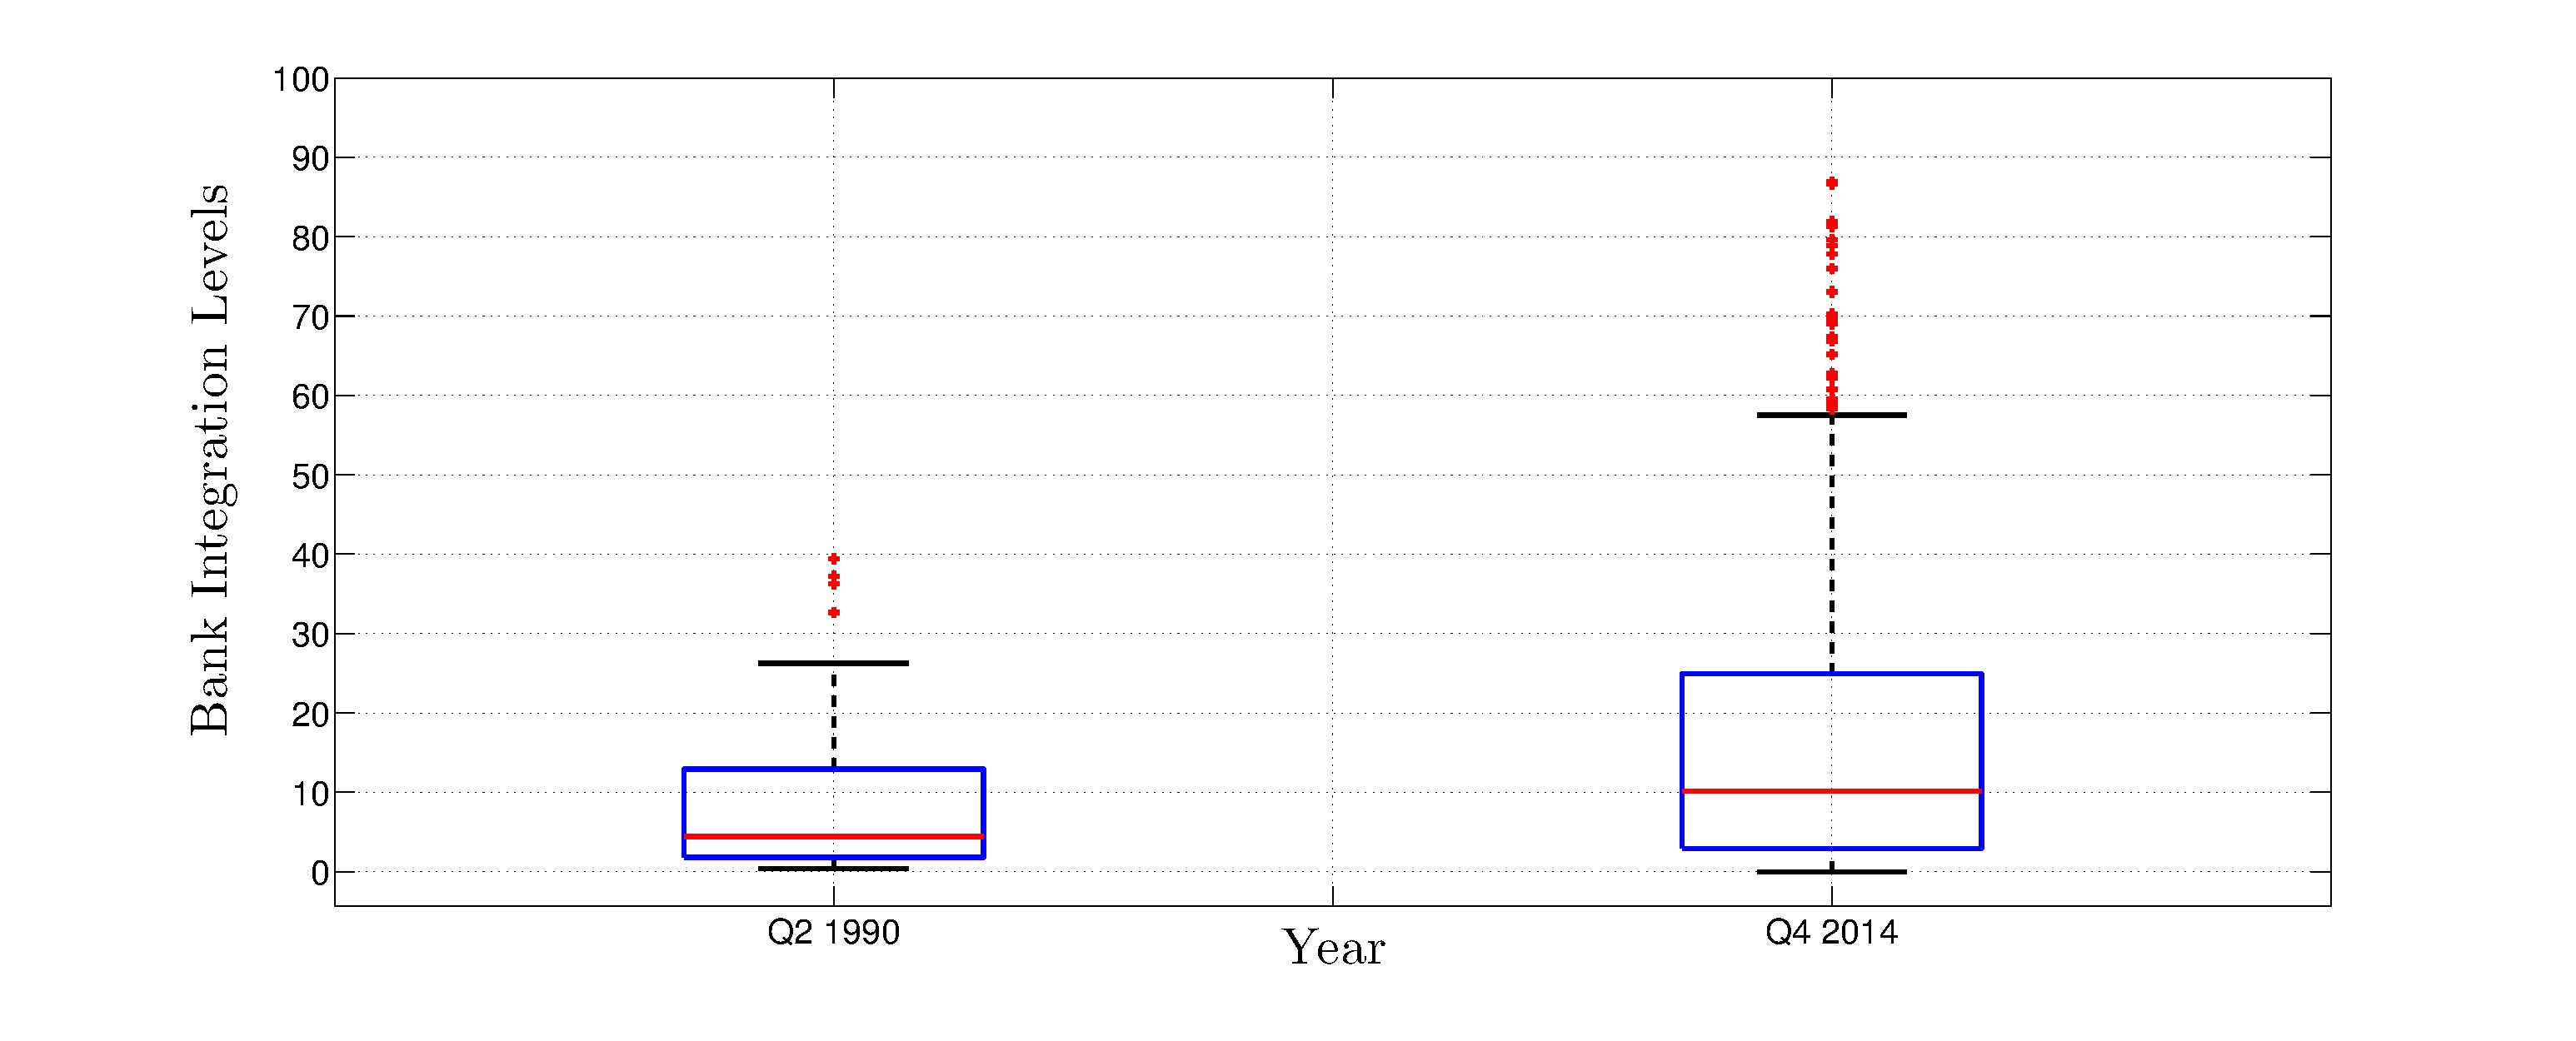
\includegraphics[width=0.5\textwidth]{Boxplot_Integration.pdf}
 	\caption{Add fancy captions here}
 	\label{Fig:Label_Boxplot} 
 \end{figure}

In general we wish to add labels to figures, sections, tables etc. since it is very
handy to be able to refer to them as and when needed using the backslash ref command.
You can use labels to refer to the section maybe a hundred pages later
by using it to go back to section \ref{Funny_Label}. 

[h!] is an option of the figure environment. This tells \LaTeX to put this image in
the next available space. Therefore if the image does not fit where it was written in
the .tex document, \LaTeX will move the float to the next page and shift some text on top of
it to minimise empty spaces. 

Another example:

 \begin{figure}[h!tbp] % htbp
 	\centering
 	%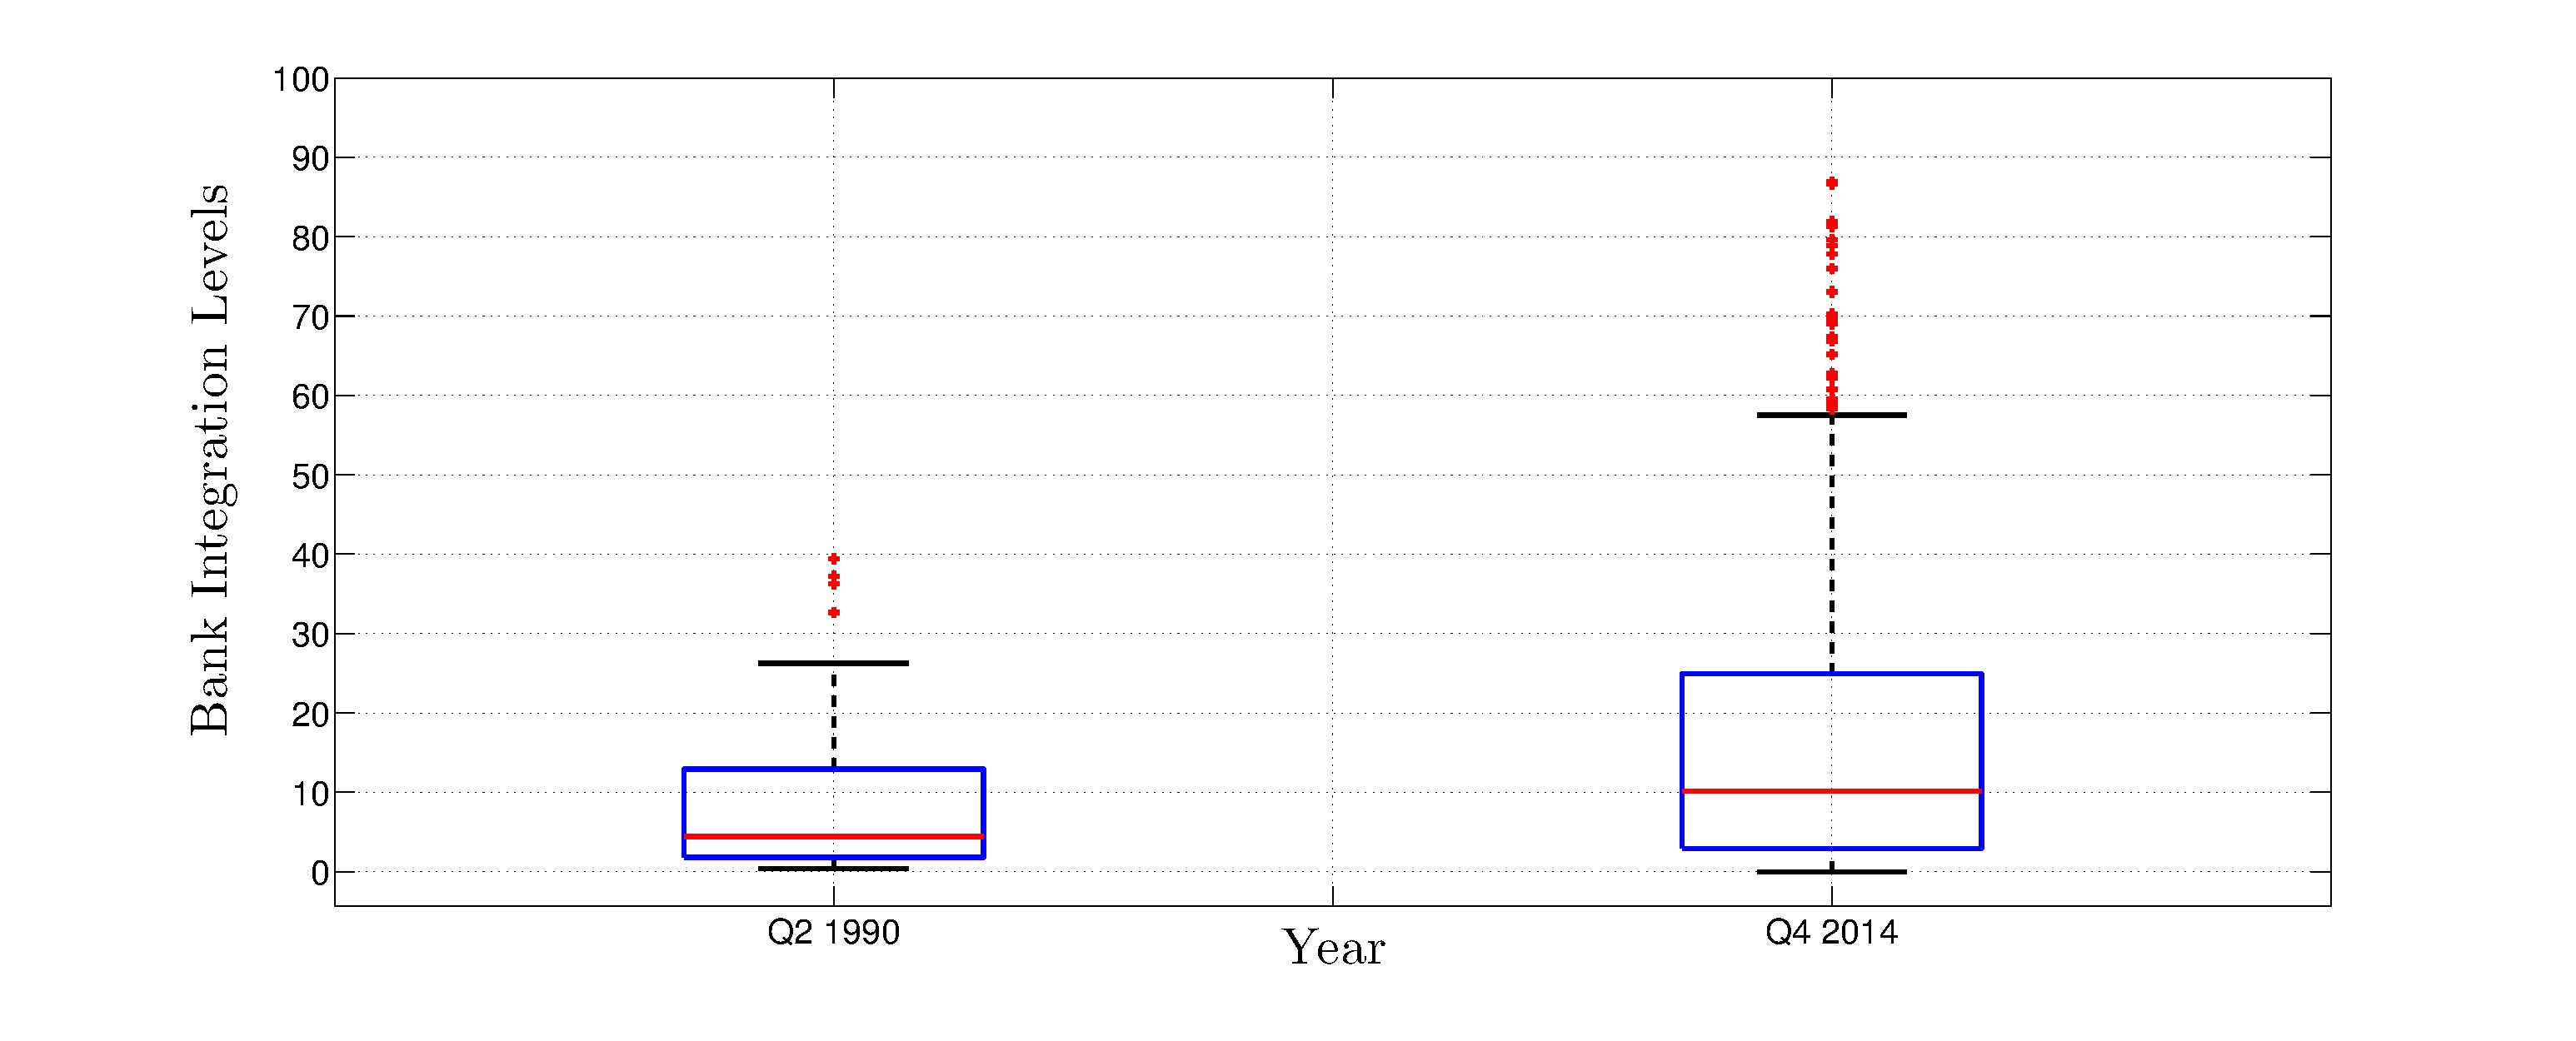
\includegraphics[width=12cm,height=6cm]{Boxplot_Integration.pdf}
 	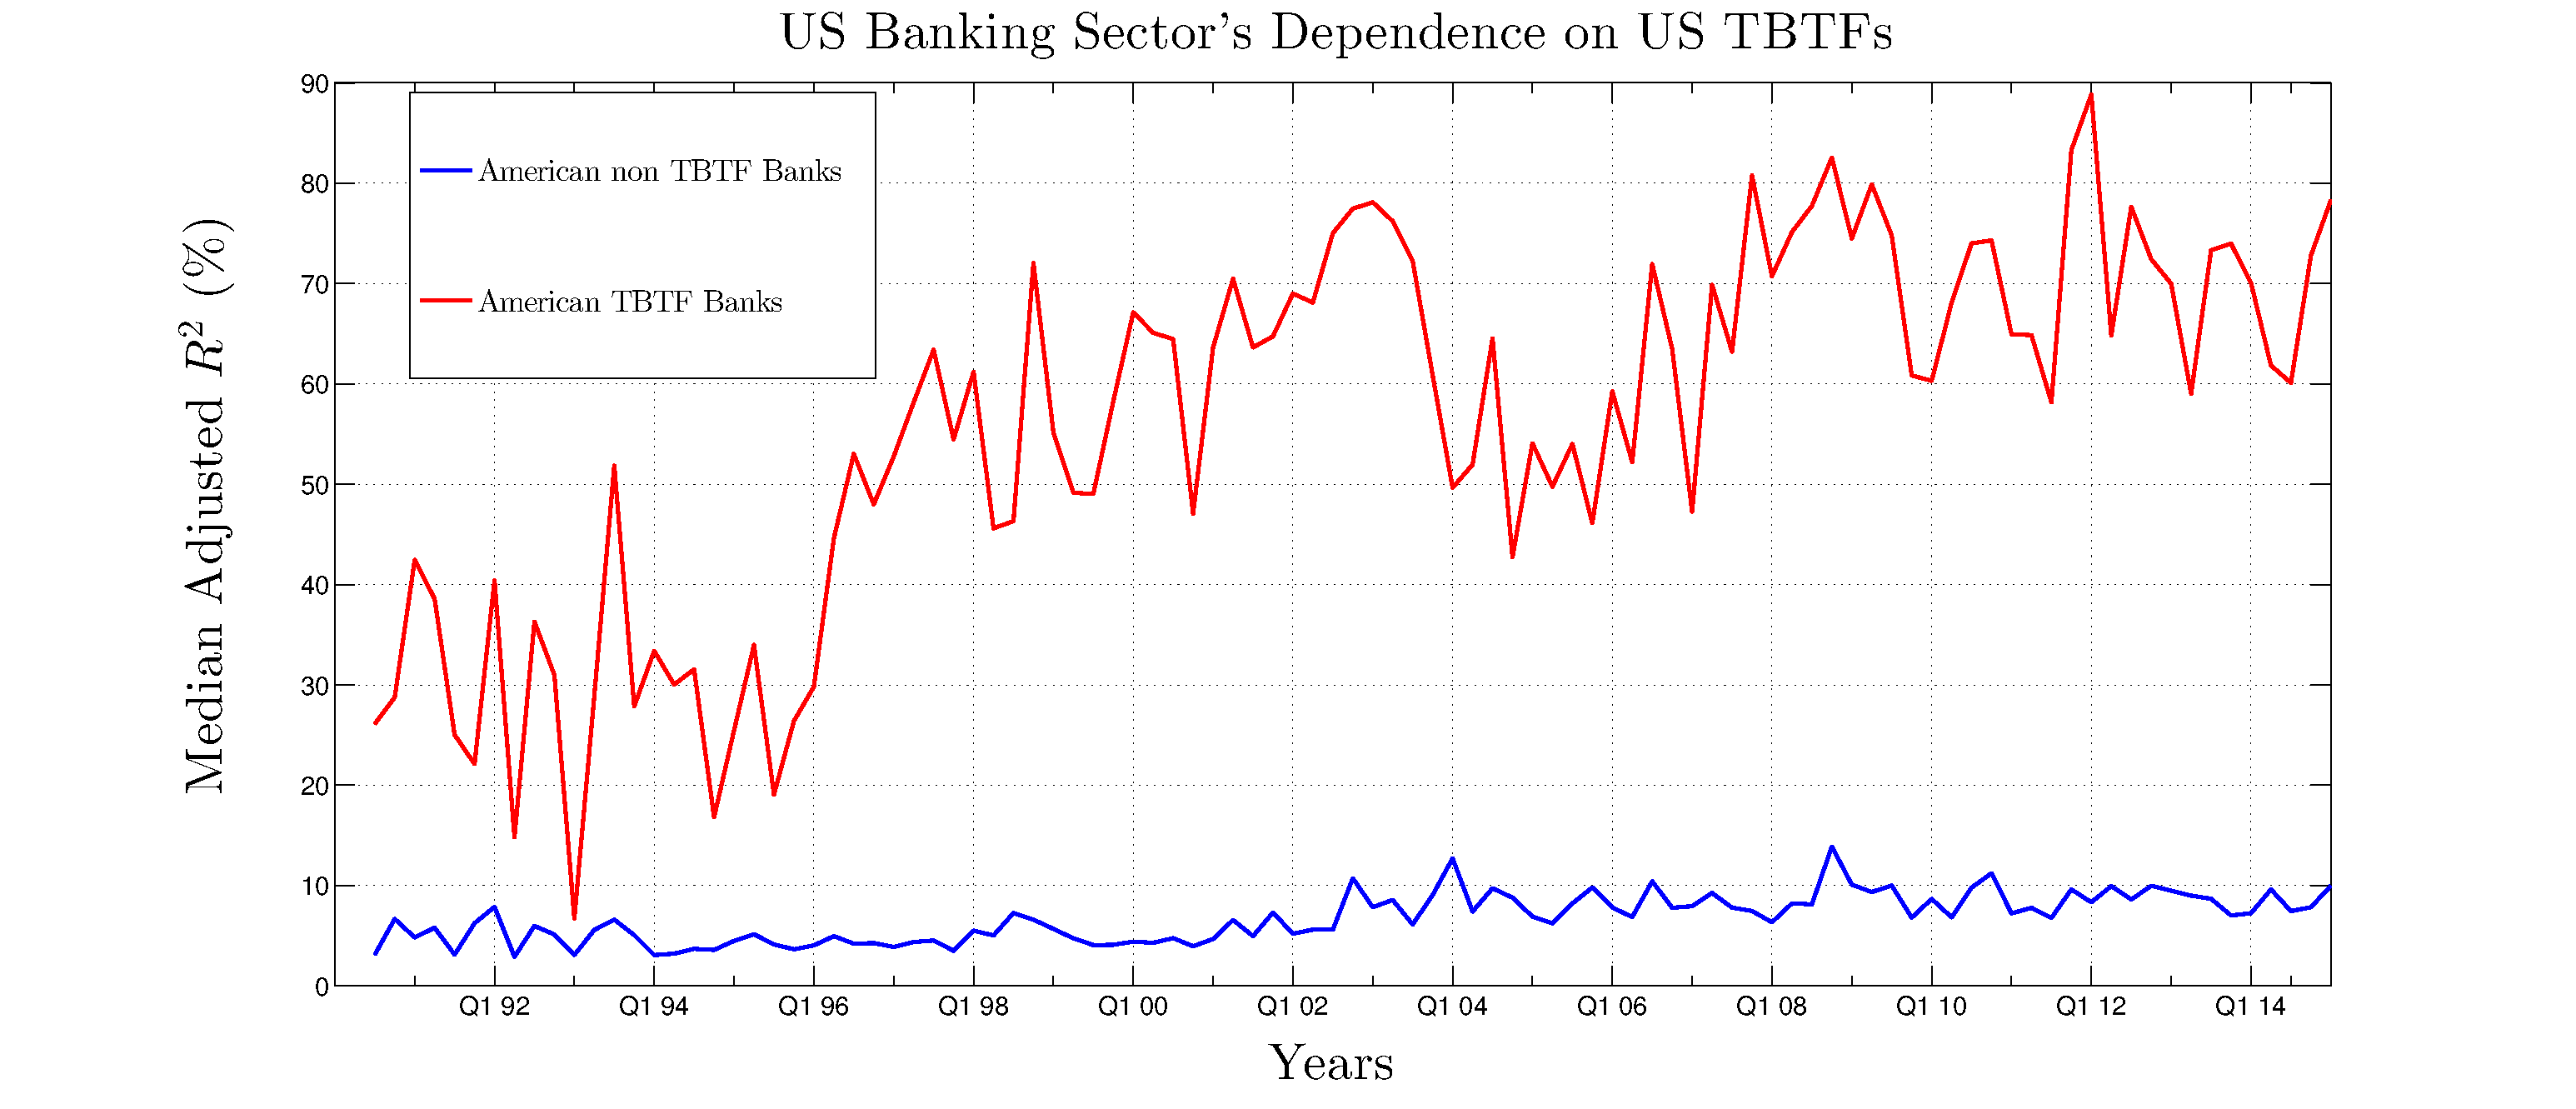
\includegraphics[width=0.9\textwidth]{Banking_Sector_US.pdf}
 	\caption{Add fancy captions here}
 	\label{Fig:Cum_fraction_eigen_US} 
 \end{figure}
 
 \section{Typeface Styles}
 
 Have a look!
 
 \subsection{Typeface}
 
 \emph{Text}, \textbf{Text}, \texttt{Text}, \textrm{Text},
 \textsf{Text}, \textsc{Text}, \textit{Text}
 
 \subsection{Size}
 
 {\tiny Text}, {\scriptsize Text}, {\footnotesize Text},
 {\small Text}, {\normalsize Text}, {\large Text}, {\Large
 	Text}, {\LARGE Text}, {\huge Text}, {\Huge Text}
 
 \subsection{Alignment}
 
 \begin{center} %/flushright/flushleft
 	put things here for fun
 \end{center} %/flushright/flushleft

\section{Lists}

There are two main types of lists that are popular --- bullet points and numbered lists

Here is how you use the bullet points:

\begin{itemize}
	\item this is one item
	\item this is another item
\end{itemize}

To generate numbered lists:

%\ref{Fig:Label_Boxplot}

\begin{enumerate}
	\item this is one item
	\item this is another item
\end{enumerate}

also, you can use whatever symbol you wish!

\begin{itemize}
	\item[$\diamond$] this is one item
	\item[$\diamond$] this is another item
\end{itemize}


\section{Tables}

\begin{table}
	\centering 
	\caption{Several types of tables can be accommodated}
	\label{Table:Systemic_Banks}
	\scriptsize{ 
		\begin{tabular}{llc} % Why lll? What about ccc or rrr or some combination?
			\hline
			&\textbf{G-SIB}			&\textbf{D-SIB} 		\\   \hline
			&Bank of America			&BB\&T					\\
			&JP Morgan Chase			&Comerica				\\
			&Wells Fargo				&Huntington Bancshares	\\
			&State Street				&M\&T Bank				\\
			&Morgan Stanley				&PNC					\\
			&Goldman Sachs				&Regions				\\
			&Bank of New York Mellon	&Zions					\\
			&Citigroup					&Fifth Third			\\
			&							&SunTrust				\\
			&							&US Bancorp				\\
			&							&KeyCorp				\\\hline
		\end{tabular}
	}
\end{table}


Let's try some more tables:

\begin{table}[ht]
	\centering
	\begin{tabular}{|r||c|c|} \hline
		Trial & $n$ & $t$ \\ \hline
		1 & 23 & 2 \\ \hline
		2 & 15 & 10 \\ \hline
		3 & 100 & 20 \\ \hline
	\end{tabular}
\end{table}

\section{References}

Finally let's see how to build bibliography:

My hero Sergiu Hart: \cite{FH:2009}

Other types of citation include \citep{FRB:2003}, \cite{Brownlees_Engle:2015},
\cite{Haas:2009}, \cite{Rachev:2005b}, \nocite{Fahlenbrach_et_al:2016} etc.



\bibliographystyle{StyWorking_Paper}% Select the citation style e.g. ieeetr
\bibliography{Introduction_to_Bibliography_Dublin_Reading_Group_20170615}% use the .bib file




\end{document}

